\subsection{Oscillatore a rilassamento}

\begin{wrapfigure}[15]{r}{0.45\textwidth}
  \begin{center}
    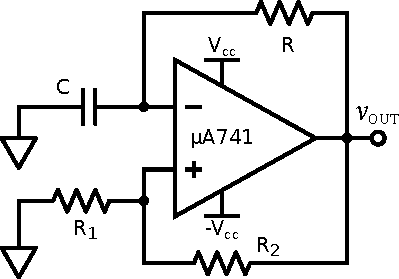
\includegraphics[width=0.30\textwidth]{../E04/latex/c_rilassamento.pdf}
  \end{center}
  \caption{Schema completo dell'oscillatore a rilassamento.}
  \label{cir4:oscillatore}
\end{wrapfigure}

In questa parte dell'esperienza studieremo il funzionamento di un oscillatore a rilassamento. Tale circuito sfrutta l'instabilità della retroazione positiva per generare un segnale oscillante con una frequenza determinata dai componenti stessi del circuito. In Figura \ref{cir4:oscillatore} è riportato lo schema circuitale. 

L'elemento circuitale fondamentale per il funzionamento dell'oscillatore a rilassamento è il condensatore C. Per comodità a $t=0$ assumiamolo scarico e $V_{out}=+V_{sat}$. Ovviamente, per effetto della retroazione negativa, la tensione all'ingresso invertente tenderà ad aumentare ($V_{inv}$ è determinata da quanta carica è accumulata sul condensatore). Non appena $|V_{inv}|>|V_{ninv}|$, avremo uno switch della tensione in uscita, ovvero $+V_{sat} \rightarrow -V_{sat}$. Il condensatore inizierà dunque a scaricarsi. Successivamente avremo un altro switch della tensione in uscita e il ciclo si ripeterà. Il periodo di tale oscillazione può essere calcolato analiticamente risolvendo il circuito. Il valore che si ottiene è $T=2RCln(1+\frac{2R_1}{R_2})$.  

Nel grafico in Figura \ref{gr4:osc10k} sono riportati i risultati ottenuti per valori di $R=\SI{9.99(1)}{\kohm}$. Come vediamo, carica e scarica del condensatore tendono a $\pm V_{sat}$.

Nella seguente tabella riportiamo i valori teorici e sperimentali di periodo dell'oscillatore a rilassamento.

\begin{center}
{\renewcommand{\arraystretch}{1.2}%
	\begin{tabular}{c|c|c}
    %\hline
	$R$ [\si{\kilo\ohm}] & $T_{exp}$ [\si{\milli\second}] & $T_{teo}$ [\si{\milli\second}]\\
    \hline
	$9.99\pm0.01 $ & $2.22\pm0.01$ & $2.19 \pm 0.03$\\
    \hline
	$99.93\pm0.01 $ & $22.2\pm0.1$ & $21.9 \pm 0.3$\\
    %\hline
	\end{tabular}
}
\end{center}

\begin{figure}[ht]
 \centering
   {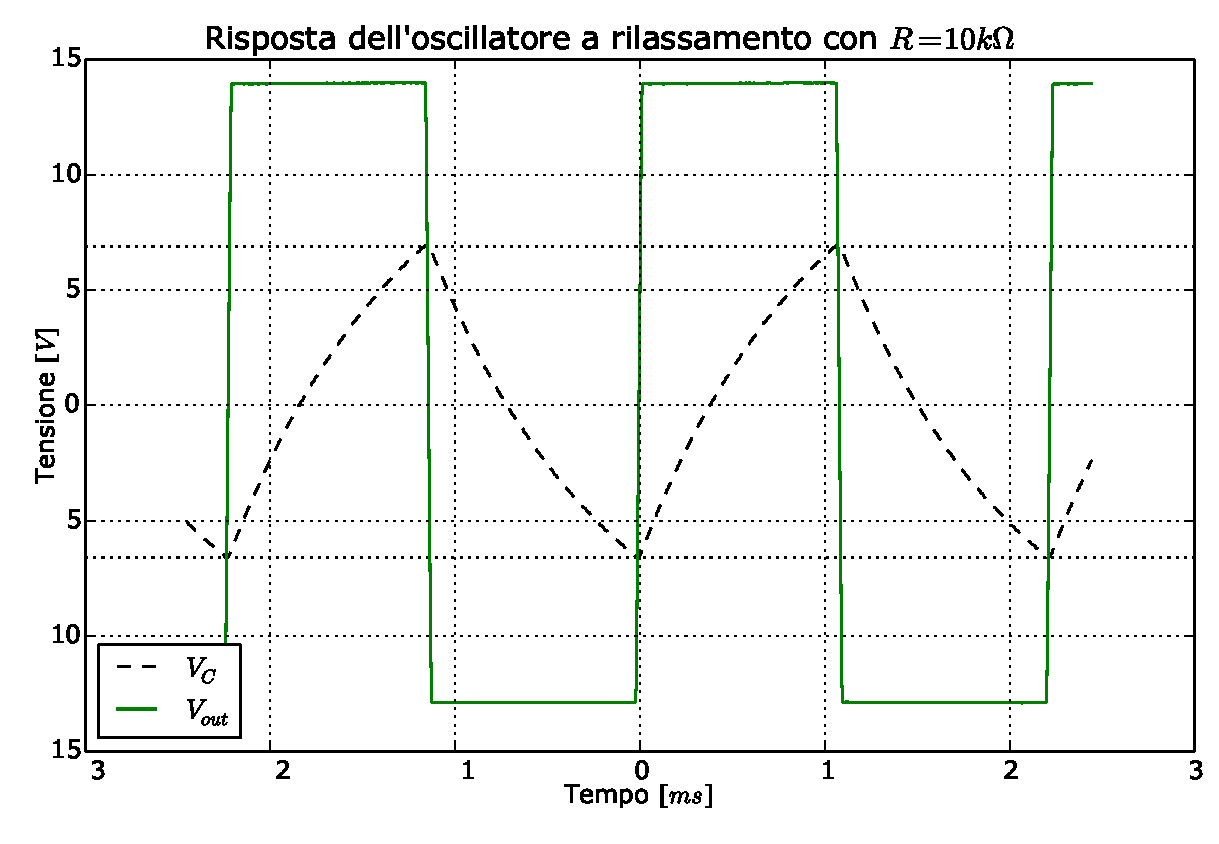
\includegraphics[width=14.5cm]{../E04/latex/osc10k.pdf}}
 \caption{Circuito oscillatore a rilassamento con $C=\SI{85.0(5)}{\nano\farad}$, $R=\SI{9.99(1)}{\kohm}$, $R_2= \SI{9.96(1)}{\kohm}$ e $R_2=\SI{9.98(1)}{\kohm}$.}
 \label{gr4:osc10k}
\end{figure}